\begin{figure}[htbp]
\centering
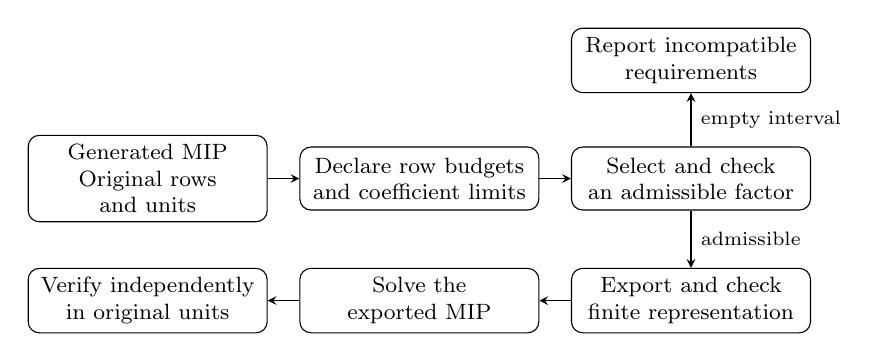
\begin{tikzpicture}[every node/.style={font=\footnotesize},
  stage/.style={draw,rounded corners,align=center,text width=2.8cm,minimum height=.8cm},
  flow/.style={->,>=stealth}]
\node[stage] (generated) at (0,0) {Generated MIP\\Original rows and units};
\node[stage] (budgets) at (3.45,0) {Declare row budgets\\and coefficient limits};
\node[stage] (select) at (6.9,0) {Select and check\\an admissible factor};
\node[stage] (export) at (6.9,-1.55) {Export and check\\finite representation};
\node[stage] (solve) at (3.45,-1.55) {Solve the\\exported MIP};
\node[stage] (verify) at (0,-1.55) {Verify independently\\in original units};
\node[stage] (abstain) at (6.9,1.5) {Report incompatible\\requirements};
\draw[flow] (generated)--(budgets);
\draw[flow] (budgets)--(select);
\draw[flow] (select)--node[right]{\scriptsize admissible}(export);
\draw[flow] (select)--node[right]{\scriptsize empty interval}(abstain);
\draw[flow] (export)--(solve);
\draw[flow] (solve)--(verify);
\end{tikzpicture}
\caption{Accuracy-aware generation and verification. A factor-selection
certificate is conditional on the exported residual; the final audit checks
the actual returned point. Neither check certifies all mixed-integer bounds.}
\label{fig:accuracy-workflow}
\end{figure}
